\section{Triển khai hệ thống}
\label{chap:trienkhai}

\begin{indentParagraph}
Chương này trình bày chi tiết quá trình triển khai hệ thống truy xuất thông tin đa phương thức từ âm thanh. Nội dung bao gồm cấu trúc dự án, triển khai các module chính, các thách thức kỹ thuật gặp phải và giải pháp, cùng với giao diện người dùng.
\end{indentParagraph}

\subsection{Cấu trúc dự án}

\subsubsection{Tổ chức thư mục}

Dự án được tổ chức theo mô hình module hóa, tách biệt rõ ràng giữa các thành phần chức năng:

\begin{lstlisting}[language=bash, caption=Cấu trúc thư mục dự án]
modules/
+-- __init__.py          # Lazy loading entry point
+-- asr_module.py        # Faster-Whisper ASR
+-- rag_module.py        # RAG + Anti-Hallucination
+-- embedding_module.py  # SBERT/E5 embeddings
+-- vector_db_module.py  # Qdrant + BM25 hybrid
+-- answer_verification.py    # Grounding check
+-- conflict_detection.py     # Date-aware conflicts
+-- post_processing.py        # OCR/ASR text cleanup
+-- prompt_templates.py       # Anti-hallucination prompts
+-- document_processor/
    +-- unified_processor.py  # 68-format factory
    +-- pdf_processor.py      # Hybrid PDF
    +-- ocr_engine.py         # PaddleOCR wrapper
    +-- audio_processor.py    # ASR integration
\end{lstlisting}

Xem cụ thể và chi tiết hơn trong: \href{https://github.com/Yudov03/DACN}{https://github.com/Yudov03/DACN}

\subsubsection{Lazy Loading Pattern}

Hệ thống sử dụng \textbf{lazy loading pattern} thông qua cơ chế \texttt{\_\_getattr\_\_} của Python để tối ưu thời gian khởi động. Các module nặng chỉ được load khi thực sự cần sử dụng:

\begin{lstlisting}[language=Python, caption=Triển khai Lazy Loading trong \_\_init\_\_.py]
# src/modules/__init__.py
def __getattr__(name):
    """Lazy import modules - only load when accessed"""
    if name == 'WhisperASR':
        from .asr_module import WhisperASR
        return WhisperASR
    elif name == 'TextEmbedding':
        from .embedding_module import TextEmbedding
        return TextEmbedding
    elif name == 'VectorDatabase':
        from .vector_db_module import VectorDatabase
        return VectorDatabase
    elif name == 'RAGSystem':
        from .rag_module import RAGSystem
        return RAGSystem
    # ... other modules
    raise AttributeError(f"module has no attribute '{name}'")
\end{lstlisting}

Kỹ thuật này giúp thời gian khởi động ứng dụng giảm từ 30 giây xuống còn 2 giây (chỉ load Streamlit UI). Khi người dùng thực hiện query đầu tiên, các module cần thiết mới được load.

\subsection{Môi trường triển khai}

% \subsubsection{Kiến trúc các thành phần}

Hệ thống bao gồm các thành phần chạy độc lập giao tiếp qua network:

% \begin{table}[H]
%     \centering
%     \caption{Các thành phần và cổng kết nối}
%     \label{tab:deployment_components}
%     \begin{tabular}{|l|l|l|p{5cm}|}
%         \hline
%         \textbf{Thành phần} & \textbf{Cổng} & \textbf{Giao thức} & \textbf{Mô tả} \\
%         \hline
%         Streamlit App & 8501 & HTTP & Student Portal UI \\
%         \hline
%         Admin Portal & 8502 & HTTP & Admin management UI \\
%         \hline
%         Qdrant & 6333 & HTTP/gRPC & Vector database \\
%         \hline
%         Ollama & 11434 & HTTP & Local LLM server \\
%         \hline
%     \end{tabular}
% \end{table}

% Hình \ref{fig:deployment_arch} minh họa kiến trúc triển khai và cách các thành phần giao tiếp với nhau:

\begin{figure}[H]
    \centering
    \begin{tikzpicture}[
        scale=0.8,
        transform shape,
        node distance=1.5cm,
        component/.style={rectangle, draw=black, fill=blue!10, minimum width=2.8cm, minimum height=1cm, align=center, rounded corners=3pt},
        database/.style={cylinder, draw=black, fill=green!10, shape border rotate=90, aspect=0.3, minimum width=2cm, minimum height=1.2cm, align=center},
        arrow/.style={->, >=stealth, thick},
        label/.style={font=\footnotesize}
    ]
        % User
        \node[component, fill=yellow!20] (user) {User\\(Browser)};

        % Streamlit Apps
        \node[component, right=2cm of user] (student) {Student Portal\\:8501};
        \node[component, above=0.8cm of student] (admin) {Admin Portal\\:8502};

        % Core modules
        \node[component, right=2cm of student, fill=orange!15] (core) {Python Core\\(RAG, ASR, Embed)};

        % External services
        \node[database, right=2cm of core] (qdrant) {Qdrant\\:6333};
        \node[component, below=0.8cm of qdrant, fill=purple!15] (ollama) {Ollama LLM\\:11434};

        % Arrows
        \draw[arrow] (user) -- node[label, above] {HTTP} (student);
        \draw[arrow] (user) |- (admin);
        \draw[arrow] (student) -- node[label, above] {import} (core);
        \draw[arrow] (admin) -| (core);
        \draw[arrow] (core) -- node[label, above] {gRPC} (qdrant);
        \draw[arrow] (core) -- node[label, right] {HTTP} (ollama);

        % Legend box
        \node[draw, dashed, fit=(student)(admin)(core), inner sep=0.3cm, label=below:{\footnotesize Python Process}] {};
    \end{tikzpicture}
    \caption{Minh họa kiến trúc triển khai và cách các thành phần giao tiếp với nhau}
    \label{fig:deployment_arch}
\end{figure}

% \subsubsection{Khởi động dịch vụ}

% Ứng dụng Streamlit tự động khởi động Ollama nếu chưa chạy, đảm bảo trải nghiệm người dùng liền mạch:

% \begin{lstlisting}[language=Python, caption=Tự động khởi động Ollama trong app.py]
% def ensure_ollama_running():
%     """Ensure Ollama is running before queries"""
%     try:
%         response = requests.get("http://localhost:11434/api/tags",
%                                 timeout=2)
%         if response.status_code == 200:
%             return True
%     except requests.exceptions.ConnectionError:
%         # Start Ollama in background
%         subprocess.Popen(["ollama", "serve"],
%                         stdout=subprocess.DEVNULL,
%                         stderr=subprocess.DEVNULL)
%         time.sleep(3)  # Wait for startup
%         return True
% \end{lstlisting}

\subsection{Triển khai module ASR}

Module ASR tích hợp Faster-Whisper với Voice Activity Detection (VAD) để xử lý audio hiệu quả. \textbf{Faster-Whisper} sử dụng CTranslate2 để tăng tốc inference lên 4x so với Whisper gốc. Module hỗ trợ \textbf{word-level timestamps} lưu trữ thời gian chính xác của từng từ để hỗ trợ trích dẫn nguồn. Tính năng \textbf{VAD filtering} (Silero VAD) tự động loại bỏ các đoạn im lặng, giảm thời gian xử lý. Đối với audio dài, hệ thống thực hiện \textbf{long audio chunking} chia thành các đoạn 30 phút để xử lý tuần tự.

Quy trình xử lý audio bắt đầu bằng việc phát hiện các đoạn có giọng nói bằng Silero VAD, sau đó chuyển đổi audio sang định dạng chuẩn (16kHz, mono). Tiếp theo, hệ thống thực hiện transcribe với word-level timestamps và cuối cùng post-process để sửa lỗi chính tả tiếng Việt.

\subsection{Triển khai module Document Processor}

Module xử lý tài liệu hỗ trợ 68 định dạng file thông qua \texttt{UnifiedProcessor}. Đây là phần mở rộng của hệ thống để tăng tính ứng dụng thực tế.

\begin{table}[H]
    \centering
    \caption{Các định dạng file được hỗ trợ}
    \label{tab:supported_formats}
    \begin{tabular}{|l|p{10cm}|}
        \hline
        \textbf{Loại} & \textbf{Định dạng} \\
        \hline
        Audio & .mp3, .wav, .m4a, .flac, .ogg, .wma, .aac \\
        \hline
        Video & .mp4, .avi, .mkv, .mov, .webm, .wmv \\
        \hline
        Document & .pdf, .docx, .doc, .txt, .md, .rtf \\
        \hline
        Spreadsheet & .xlsx, .xls, .csv \\
        \hline
        Presentation & .pptx, .ppt \\
        \hline
        Image & .png, .jpg, .jpeg, .tiff, .bmp (OCR) \\
        \hline
        Code & .py, .js, .java, .cpp, .go, .rs (30+ ngôn ngữ) \\
        \hline
    \end{tabular}
\end{table}

Hệ thống sử dụng các thư viện chuyên biệt cho từng loại file thay vì tự xây dựng parser. Cụ thể: \texttt{python-docx} cho Word, \texttt{openpyxl} cho Excel, \texttt{python-pptx} cho PowerPoint, \texttt{PaddleOCR} cho hình ảnh, và \texttt{Faster-Whisper} cho audio/video. Kiến trúc Factory Pattern (\texttt{UnifiedProcessor}) cho phép dễ dàng mở rộng thêm định dạng mới.

\textbf{Hybrid PDF Processing:} Hệ thống sử dụng chế độ hybrid cho PDF, kết hợp text extraction và OCR. Với mỗi trang, hệ thống đánh giá tỷ lệ text/image để quyết định phương pháp xử lý phù hợp, tăng tốc độ 10x so với full-page OCR.

\subsection{Triển khai hệ thống RAG}

\subsubsection{Query Processing Pipeline}

Pipeline xử lý truy vấn được thiết kế theo chuỗi các bước xử lý tuần tự, mỗi bước đóng góp vào việc cải thiện chất lượng câu trả lời cuối cùng. Khi nhận được câu hỏi từ người dùng, hệ thống trước tiên thực hiện Query Expansion để mở rộng câu hỏi gốc với các từ đồng nghĩa và biến thể, tăng khả năng tìm được tài liệu liên quan. Câu hỏi đã mở rộng sau đó được sử dụng cho Hybrid Search kết hợp vector search tìm kiếm theo ngữ nghĩa và BM25 tìm kiếm theo từ khóa, kết quả từ hai phương pháp được gộp lại bằng Reciprocal Rank Fusion.

Danh sách kết quả sơ bộ được đưa qua Reranking sử dụng cross-encoder để sắp xếp lại theo độ liên quan chính xác hơn. Trước khi sinh câu trả lời, Conflict Detection phân tích các nguồn tìm được để phát hiện mâu thuẫn và xử lý theo chiến lược đã cấu hình. Answer Generation sử dụng LLM để sinh câu trả lời dựa trên context đã được lọc và xử lý, kèm theo prompt template được thiết kế để giảm thiểu hallucination. Bước cuối cùng là Answer Verification kiểm chứng tính chính xác của câu trả lời dựa trên nguồn gốc và gán mức độ tin cậy phù hợp.

\subsubsection{Anti-Hallucination Mechanisms}

Hệ thống triển khai ba cơ chế chống ảo giác:

\begin{table}[H]
    \centering
    \caption{Cơ chế chống ảo giác}
    \label{tab:anti_halluc_mechanisms}
    \begin{tabular}{|l|p{4cm}|p{6cm}|}
        \hline
        \textbf{Cơ chế} & \textbf{Chức năng} & \textbf{Cách hoạt động} \\
        \hline
        Answer Verification & Kiểm chứng câu trả lời & So sánh câu trả lời với nguồn, phân loại mức độ grounding \\
        \hline
        Conflict Detection & Phát hiện mâu thuẫn & Phân tích ngày tháng và nội dung, ưu tiên thông tin mới \\
        \hline
        Safe Abstention & Từ chối trả lời & Không trả lời khi không đủ thông tin, gợi ý câu hỏi phù hợp \\
        \hline
    \end{tabular}
\end{table}

\subsubsection{Prompt Engineering}

Prompt được thiết kế để giảm thiểu hallucination với các quy tắc nghiêm ngặt. Dưới đây là prompt template \texttt{strict\_qa} được sử dụng mặc định:

\begin{lstlisting}[language=Python, caption=Prompt template strict\_qa cho Anti-Hallucination]
# src/modules/prompt_templates.py
self.templates["strict_qa"] = PromptTemplate(
    name="strict_qa",
    description="Anti-hallucination template - citation required",
    system_prompt="""You are a STRICT AI assistant. MANDATORY rules:

1. ONLY answer from information IN the provided context
2. EVERY piece of information MUST have a citation [Source X]
3. DO NOT infer, assume, or add external information
4. If information NOT FOUND -> answer EXACTLY:
   "No information found in the documents."
5. If information is INCOMPLETE -> only answer what's available,
   clearly state what's missing

ABSOLUTELY DO NOT:
- Make up information not in context
- Use general knowledge
- Assume or infer beyond what's stated""",
    user_prompt="""Context:
{context}

Question: {question}

Answer (ONLY from context, with citations):""",
    variables=["context", "question"]
)
\end{lstlisting}

Template \texttt{safe\_abstention} được sử dụng khi cần ưu tiên độ chính xác cao:

\begin{lstlisting}[language=Python, caption=Prompt template safe\_abstention]
self.templates["safe_abstention"] = PromptTemplate(
    name="safe_abstention",
    description="Safe template - refuse when uncertain",
    system_prompt="""You are an AI that PRIORITIZES ACCURACY over completeness.

GOLDEN RULES:
1. Only answer when CONFIDENCE >= 80%
2. If only partial info -> answer that part, note what's missing
3. If UNCERTAIN -> respond:
   "I cannot find sufficient information to answer this question.
    [If related info exists: May be related: ...]
    [Suggest alternative question or request more documents]"

It is BETTER to say "I don't know" than to guess.""",
    ...
)
\end{lstlisting}

\subsection{Triển khai Post-Processing với Cache}

Module Post-Processing sử dụng LLM để sửa lỗi chính tả và chuẩn hóa văn bản từ ASR/OCR. Để tránh xử lý lại nội dung đã xử lý, hệ thống triển khai caching với MD5 hash:

\begin{lstlisting}[language=Python, caption=Triển khai MD5 Cache Key trong post\_processing.py]
# src/modules/post_processing.py
import hashlib

class PostProcessingCache:
    def _generate_key(self, text: str, method: str, model: str) -> str:
        content = f"{text}|{method}|{model}"
        return hashlib.md5(content.encode('utf-8')).hexdigest()

    def get(self, text: str, method: str, model: str) -> Optional[str]:
        """Get cached result if exists"""
        cache_key = self._generate_key(text, method, model)
        cache_file = self.cache_dir / f"{cache_key}.json"
        if cache_file.exists():
            with open(cache_file, 'r', encoding='utf-8') as f:
                return json.load(f)["result"]
        return None
\end{lstlisting}

\begin{table}[H]
    \centering
    \caption{Hiệu quả của Post-Processing Cache}
    \label{tab:cache_stats}
    \begin{tabular}{|l|c|}
        \hline
        \textbf{Metric} & \textbf{Giá trị} \\
        \hline
        Cache key format & MD5(method:model:content) \\
        Cache hit rate (re-index) & 95\% \\
        Thời gian xử lý (cache miss) & 5-30 giây/chunk \\
        Thời gian xử lý (cache hit) & 0.01 giây/chunk \\
        Tiết kiệm thời gian re-index & 93\% \\
        \hline
    \end{tabular}
\end{table}

\subsection{Triển khai Vector Database}

Hệ thống sử dụng Qdrant làm vector database với \textbf{HNSW Index} cho tìm kiếm approximate nearest neighbors nhanh và \textbf{Cosine Similarity} làm độ đo khoảng cách cho embedding vectors. \textbf{Payload Storage} lưu trữ metadata bao gồm source, timestamps và file type. \textbf{BM25 Index} được xây dựng riêng cho keyword search. Hybrid search kết hợp vector search và BM25 bằng Reciprocal Rank Fusion (RRF), cải thiện MRR từ 0.62 lên 0.75.

\subsection{Triển khai giao diện người dùng}

\subsubsection{Student Portal}

\begin{figure}[H]
    \centering
    \includegraphics[width=0.9\textwidth]{report/figures/Student Portal.png}
    \caption{Student Portal Screen}
    \label{fig:Student Portal}
\end{figure}

% Giao diện chat cho sinh viên tra cứu thông tin với hai phương thức nhập liệu: văn bản và giọng nói. Thanh nhập liệu gồm ô text input và nút Voice Input. Câu trả lời được hiển thị kèm verification status cho biết mức độ tin cậy. Sinh viên có thể xem nguồn tham khảo với timestamps và nghe câu trả lời bằng TTS tiếng Việt.



\subsubsection{Voice Input}

Voice Input cho phép sinh viên đặt câu hỏi bằng giọng nói, tạo trải nghiệm hỏi đáp hoàn toàn bằng âm thanh khi kết hợp với TTS. Hệ thống sử dụng thư viện \texttt{audio-recorder-streamlit} để ghi âm từ microphone của browser, sau đó tái sử dụng module WhisperASR đã có để chuyển đổi thành văn bản.

Luồng xử lý Voice Input gồm 5 bước: (1) Người dùng nhấn nút microphone và nói câu hỏi, (2) Browser thu âm qua microphone và trả về audio bytes, (3) Audio được lưu tạm thành file WAV và gửi đến WhisperASR, (4) Transcript được hiển thị để người dùng xác nhận, (5) Query được xử lý qua RAG pipeline và câu trả lời tự động được đọc bằng TTS.

% Hình \ref{fig:voice_sequence} thể hiện sơ đồ trình tự (Sequence Diagram) của luồng Voice-to-Voice, cho thấy độ trễ tại mỗi bước xử lý:

\begin{figure}[H]
    \centering
    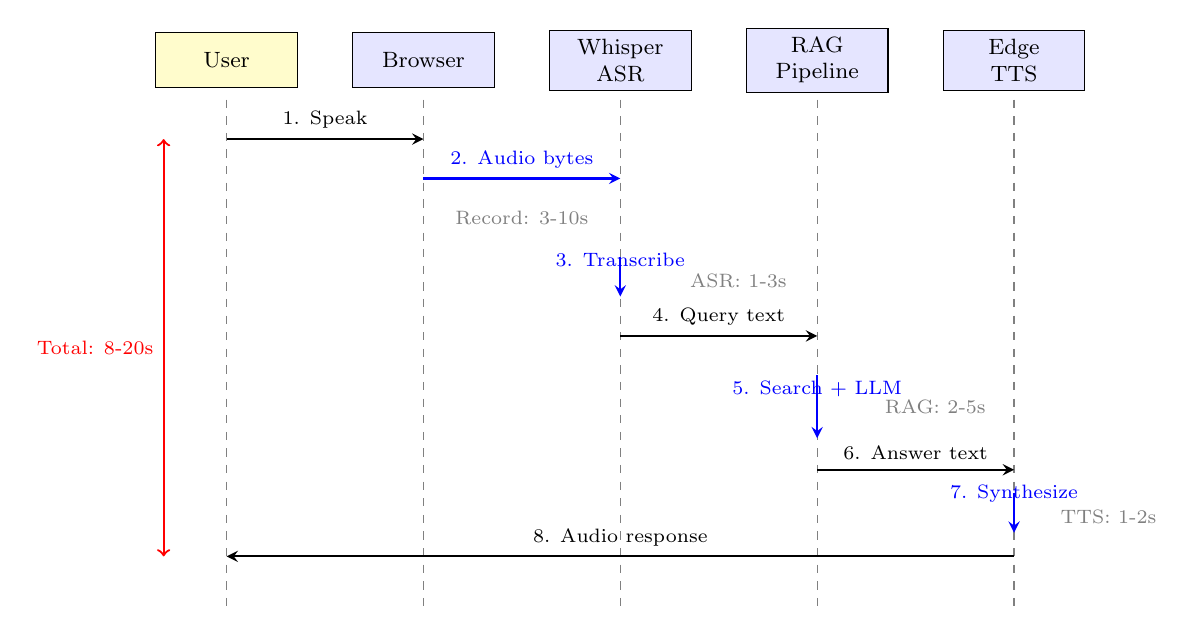
\begin{tikzpicture}[
        actor/.style={rectangle, draw=black, fill=yellow!20, minimum width=1.8cm, minimum height=0.7cm, align=center, font=\footnotesize},
        component/.style={rectangle, draw=black, fill=blue!10, minimum width=1.8cm, minimum height=0.7cm, align=center, font=\footnotesize},
        arrow/.style={->, >=stealth, thick},
        note/.style={font=\scriptsize, text=gray}
    ]
        % Actors/Components (top row)
        \node[actor] (user) at (0,0) {User};
        \node[component] (browser) at (2.5,0) {Browser};
        \node[component] (whisper) at (5,0) {Whisper\\ASR};
        \node[component] (rag) at (7.5,0) {RAG\\Pipeline};
        \node[component] (tts) at (10,0) {Edge\\TTS};

        % Lifelines
        \foreach \x in {0, 2.5, 5, 7.5, 10} {
            \draw[dashed, gray] (\x, -0.5) -- (\x, -7);
        }

        % Messages
        \draw[arrow] (0, -1) -- node[above, font=\scriptsize] {1. Speak} (2.5, -1);
        \draw[arrow, blue] (2.5, -1.5) -- node[above, font=\scriptsize] {2. Audio bytes} (5, -1.5);
        \node[note] at (3.75, -2) {Record: 3-10s};

        \draw[arrow, blue] (5, -2.5) -- node[above, font=\scriptsize] {3. Transcribe} (5, -3);
        \node[note] at (6.5, -2.8) {ASR: 1-3s};

        \draw[arrow] (5, -3.5) -- node[above, font=\scriptsize] {4. Query text} (7.5, -3.5);

        \draw[arrow, blue] (7.5, -4) -- node[above, font=\scriptsize] {5. Search + LLM} (7.5, -4.8);
        \node[note] at (9, -4.4) {RAG: 2-5s};

        \draw[arrow] (7.5, -5.2) -- node[above, font=\scriptsize] {6. Answer text} (10, -5.2);

        \draw[arrow, blue] (10, -5.5) -- node[above, font=\scriptsize] {7. Synthesize} (10, -6);
        \node[note] at (11.2, -5.8) {TTS: 1-2s};

        \draw[arrow] (10, -6.3) -- node[above, font=\scriptsize] {8. Audio response} (0, -6.3);

        % Total latency
        \draw[<->, thick, red] (-0.8, -1) -- node[left, font=\scriptsize, text=red] {Total: 8-20s} (-0.8, -6.3);

    \end{tikzpicture}
    \caption{Sơ đồ trình tự Voice-to-Voice với độ trễ tại mỗi bước}
    \label{fig:voice_sequence}
\end{figure}

Tính năng Auto-TTS cho phép bật/tắt trong sidebar. Khi bật, hệ thống tự động đọc câu trả lời mỗi khi nhận được truy vấn bằng giọng nói, tạo trải nghiệm hands-free hoàn toàn.

\subsubsection{Admin Portal}


\begin{figure}[H]
    \centering
    \includegraphics[width=0.9\textwidth]{report/figures/Admin Portal.png}
    \caption{Admin Portal Screen}
    \label{fig:Admin Portal}
\end{figure}
% Giao diện quản lý cho quản trị viên với Dashboard thống kê tổng quan về tài liệu, chunks và loại file. Chức năng Upload tài liệu hỗ trợ drag-and-drop và xử lý batch nhiều file cùng lúc. Quản trị viên có thể xem, xóa, re-index từng file riêng lẻ. Phần cấu hình hệ thống cho phép thay đổi model và chunking method.

\subsection{Các thách thức kỹ thuật và giải pháp}

\begin{table}[H]
    \centering
    \caption{Các thách thức kỹ thuật và giải pháp}
    \label{tab:technical_challenges}
    \begin{tabular}{|p{3.5cm}|p{4.5cm}|p{5.5cm}|}
        \hline
        \textbf{Thách thức} & \textbf{Vấn đề} & \textbf{Giải pháp} \\
        \hline
        GPU Memory (OOM) & Xử lý audio dài >60 phút gây tràn VRAM với model Whisper large & Chia audio thành chunks 30 phút; Hỗ trợ chọn model size (tiny/base/small) qua .env; Tự động fallback về CPU khi GPU không đủ bộ nhớ \\
        \hline
        OCR không ra chữ & Hình ảnh chất lượng thấp, scan mờ, nghiêng & Tiền xử lý ảnh (resize, denoise, deskew); Giới hạn kích thước ảnh tối đa 3500px để tránh crash PaddleOCR \\
        \hline
        Thời gian khởi động & Load tất cả models mất 30+ giây & Lazy loading pattern - chỉ load module khi cần; Giảm startup xuống 2 giây \\
        \hline
        LangChain compatibility & PaddleOCR dùng langchain 0.x imports đã deprecated & Tạo compatibility shim trong \_\_init\_\_.py redirect imports về langchain\_core \\
        \hline
        Tiếng Việt encoding & Windows terminal không hiển thị đúng tiếng Việt & Thiết lập UTF-8: chcp 65001; Sử dụng encoding='utf-8' trong tất cả file I/O \\
        \hline
        Re-index tốn thời gian & Mỗi lần đổi config phải re-process từ đầu & Cache MD5 cho post-processing; Tách 2 bước: process (OCR/ASR) và reindex (embed) \\
        \hline
    \end{tabular}
\end{table}

% Đoạn code xử lý long audio chunking:

% \begin{lstlisting}[language=Python, caption=Xử lý audio dài với chunking]
% # src/modules/asr_module.py
% def transcribe_long_audio(self, audio_path: str,
%                           chunk_duration: int = 1800):  # 30 minutes
                          
%     audio = AudioSegment.from_file(audio_path)
%     duration_ms = len(audio)
%     chunk_ms = chunk_duration * 1000

%     all_segments = []
%     for start_ms in range(0, duration_ms, chunk_ms):
%         end_ms = min(start_ms + chunk_ms, duration_ms)
%         chunk = audio[start_ms:end_ms]

%         # Export chunk to temp file
%         temp_path = f"/tmp/chunk_{start_ms}.wav"
%         chunk.export(temp_path, format="wav")

%         # Transcribe chunk
%         segments = self.transcribe(temp_path)

%         # Adjust timestamps
%         for seg in segments:
%             seg["start"] += start_ms / 1000
%             seg["end"] += start_ms / 1000
%         all_segments.extend(segments)

%     return all_segments
% \end{lstlisting}

\newpage
\subsection*{Tổng kết triển khai}

Hệ thống đã được triển khai thành công với đầy đủ các thành phần theo thiết kế đề ra. Module ASR sử dụng Faster-Whisper kết hợp Silero VAD để nhận dạng giọng nói tiếng Việt với khả năng lưu giữ word-level timestamps phục vụ cho việc trích dẫn nguồn. Document Processor với UnifiedProcessor hỗ trợ 68 định dạng file thông qua các thư viện chuyên biệt, trong đó PDF được xử lý theo chế độ hybrid kết hợp text extraction và OCR để tối ưu cả tốc độ và độ chính xác.

RAG System là thành phần trung tâm tích hợp hybrid search và hệ thống anti-hallucination đa tầng với các prompt templates được thiết kế cẩn thận. Module Post-Processing sử dụng LLM để sửa lỗi chính tả kết hợp với cơ chế caching MD5 hash giúp tiết kiệm đáng kể thời gian khi re-index. Qdrant đóng vai trò làm vector database với khả năng kết hợp BM25 cho hybrid search.

Voice Input được triển khai dựa trên thư viện audio-recorder-streamlit để thu âm từ browser, tái sử dụng module WhisperASR đã có để chuyển đổi thành văn bản. Kết hợp với Edge-TTS đọc câu trả lời bằng giọng tiếng Việt, hệ thống tạo nên trải nghiệm hỏi đáp hoàn toàn bằng âm thanh - một tính năng đặc biệt hữu ích trong nhiều ngữ cảnh sử dụng. Giao diện web bao gồm Student Portal cho sinh viên tra cứu thông tin và Admin Portal cho quản trị viên quản lý tài liệu.

Quá trình triển khai đã giải quyết thành công các thách thức kỹ thuật như xử lý audio dài (chunking 30 phút), tối ưu thời gian khởi động (lazy loading), và đảm bảo tương thích với các thư viện cũ (compatibility shim). Mã nguồn được tổ chức theo mô hình module hóa, hệ thống có thể hoạt động hoàn toàn offline với Ollama và các mô hình embedding cục bộ, đáp ứng yêu cầu về chi phí và bảo mật dữ liệu.

\newpage
